\documentclass[]{article}

% Imported Packages
%------------------------------------------------------------------------------
\usepackage{amssymb}
\usepackage{amstext}
\usepackage{amsthm}
\usepackage{amsmath}
\usepackage{enumerate}
\usepackage{fancyhdr}
\usepackage{float}
\usepackage[margin=1in]{geometry}
\usepackage{graphicx}
\usepackage{extarrows}
\usepackage{setspace}
\usepackage{indentfirst}
%------------------------------------------------------------------------------

% Header and Footer
%------------------------------------------------------------------------------
\pagestyle{plain}  
\renewcommand\headrulewidth{0.4pt}                                      
\renewcommand\footrulewidth{0.4pt}                                    
%------------------------------------------------------------------------------

% Title Details
%------------------------------------------------------------------------------
\title{Deliverable \#1}
\author{SE 3A04: Software Design II -- Large System Design}
\date{February 5, 2021}                               

%------------------------------------------------------------------------------
\begin{document}

\maketitle	

\section{Introduction}
\label{sec:introduction}
% Begin Section 1
The \textbf{SRS} will give an overall description of the project. This overview will include the functional, non-functional and performance requirements, and a use case diagram of the application. These will describe what the software will do and how it will be expected to perform.

\subsection{Purpose}
\label{sub:purpose}
% Begin Subsection
The purpose of this project is to build an interactive computer game which involves the user fixing various parts of a ship through mini-games to reach an undefined location. The story line of this game follows a saboteur that has wrecked various parts of the ship, which the player must fix to save everyone on board.

This game has been designed in a way to be playable for any general audience that can understand and grasp basic game mechanics.
% End Subsection

\subsection{Scope}
\label{sub:scope}
% Begin Subsection
This product will be a Web-based JavaScript game. The game will include 5 mini-games to choose from on a main screen, where the user will be able to move and click on a game they choose to play. The game will not include any save progress of the player, or include any account creation process. The player must restart the game if they refresh or exit the server.
\\

The game is intended to be a Web-based game programmed in JavaScript. The benefits to using JavaScript is that there is a large community and help surrounding web applications built in JavaScript, as it is one of the most popular languages for website development. It would also be beneficial to make use of a popular JavaScript \textbf{Web Framework} such as React or Angular, or other popular frameworks. A framework would provide an easy way to create a robust back-end and attractive front-end interface. Another goal is to also host the server using a free cloud-based development platform, such as Heroku or Firebase.
% End SubSection

\subsection{Definitions, Acronyms, and Abbreviations}
\label{sub:definitions_acronyms_and_abbreviations}
% Begin SubSection
\begin{itemize}
    \item SRS: Software Requirement Specification
    \item API: Application Programming Interface
    \item HTML: Hyper Text Markup Language
    \item CSS: Cascading Style Sheets
    \item WCAG: Web Content Accessibility Guidelines
    \item Web Framework: Created to support the development of dynamic web applications
\end{itemize}
% End Subsection
\newpage
\subsection{References}
\label{label:references}
\bibliographystyle{plain}
\bibliography{references}

\subsection{Overview}
\label{sub:overview}
% Begin Subsection
The SRS will define the business requirements of the system and its functional and non-functional requirements through various viewpoints. 
\\

The SRS is split into five sections. The first section is the introduction and overview of the SRS. Section 2 is an overall description of the product. Section 3 demonstrates a use case diagram for the application. Section 4 states the functional requirements, and Section 5 states the non-functional requirements.
% End Subsection

% End Section 1

\section{Overall Description}
\label{sec:overall_description}
% Begin Section 2
\subsection{Product Perspective}
\label{sub:product_perspective}
% Begin Subsection
The product is related to the popular online multiplayer social deduction game \textit{Among Us}, as they have similar themes. Both games have a "core" and some "mini-games". Players need to complete all of these mini-games to finish the game. The product is not totally self-contained, the mini-games will require use of external \textbf{APIs}. Specifically for the trivia mini-game, an \textbf{API} will be used to pull trivia questions and answers for the user.
\\

Since the product is to be hosted on a cloud-based development platform, there are many components that will be handled without the need of a developer being involved in the hosting process. Therefore, it is only necessary for the system to deploy the content and design of the website, which is the Document Object Model. The block diagram of the game is presented as follows:
\newpage
\begin{figure}[H]
    \centering
    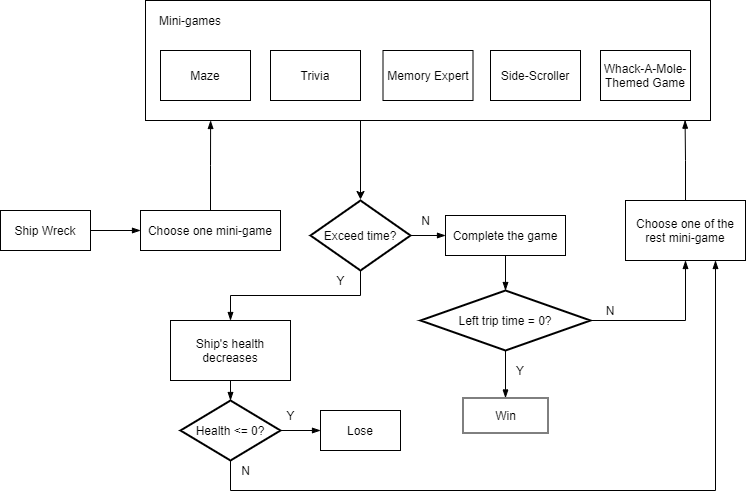
\includegraphics[width=1\textwidth]{figures/BlockDiagram.png}
    \caption{Block diagram of the project}
\end{figure}
% End Subsection


\subsection{Product Functions}
\label{sub:product_functions}
% Begin Subsection
The user can start a game, choose a difficulty and adjust the sound of the game. When the game starts, their in-game character will be placed in a ship. 

\bigskip
\textit{The user will be able to complete tasks via playing a variety of mini-games on this ship. The level of difficulty coincides with the one chosen at the start of the game. Each of these mini-games have varying requirements that the user must accomplish.}
\bigskip 

There are five mini-games that the user can play. These five games involve:
\begin{itemize}
    \item A maze
    \item Trivia
    \item Memory expert
    \item Side-scroller
    \item Whack-A-Mole-themed game
\end{itemize}
If the user fails to complete a task, their ship takes an arbitrary amount of damage, decreasing the ship's durability. If the durability value of the ship reaches 0, the ship crashes, and the user loses the game. If the ship's durability remains above 0 for a pre-specified period of time, the user wins the game. This pre-specified period is defined by the difficulty of the game.

% End Subsection

\subsection{User Characteristics}
\label{sub:user_characteristics}
% Begin Subsection
A technical background is not necessary to run or play the game. It should be playable for anyone with knowledge of simple keyboard and mouse operations in order to complete the mini-game components.
\\


As this game is based on \textit{Among Us}, the intended audience would be the same as those who have played \textit{Among Us} or are familiar with the game.
\\


An educational background is not necessary to play this game. Experience with games with similar themes to the mini-games is beneficial to the user's success, but not crucial to playing the game itself.
    
\subsection{Constraints}
\label{sub:constraints}
% Begin Subsection
\begin{itemize}
	\item Cost: Tools that do not require purchasing a service are used within the project, as they are great free alternatives to achieving the overall goal.
	\item Scope: The scope of the project only includes creating 5 mini-games, where the user will be redirected to whichever game they choose to click on.
	\item Resources: Simply choosing to create this project as a web application restricts the tools developers are able to use. Certain languages are not likely to be used for web applications, such as Haskell or C\#. It is preferable to use a language that is well-known and provides more support in case of any problems in achieving a task.
\end{itemize}
% End Subsection

\subsection{Assumptions and Dependencies}
\label{sub:assumptions_and_dependencies}
% Begin Subsection
The following assumptions and dependencies are stated below:
\begin{itemize}
	\item Based on the browser used for the web application, the  \textbf{HTML} and  \textbf{CSS} might be affected. This project will use the assumption that a user will be using the latest version of Google Chrome.
	\item The user must have a stable internet connection in order to efficiently play the game, considering that a page refresh will cause all game progress to be lost.
	\item The user has proficiency in the English language.
\end{itemize}
% End Subsection

\subsection{Apportioning of Requirements}
\label{sub:apportioning_of_requirements}
% Begin Subsection
As the user base grows, it will be required to upgrade the server capacity to support more simultaneous requests. Building a scalable architecture will be a requirement, but supporting a high number of requests will not be necessary until later in the project.
\\


Monetization will also be a future requirement and is not a priority right away. But over the long term, there will need to be a source of revenue which may come from running advertisements or adding in-game micro transactions users can purchase.
% End Subsection

% End Section 2

\section{Use Case Diagram}
\label{sec:use_case_diagram}
% Begin Section 3
\begin{figure}[H]
    \centering
    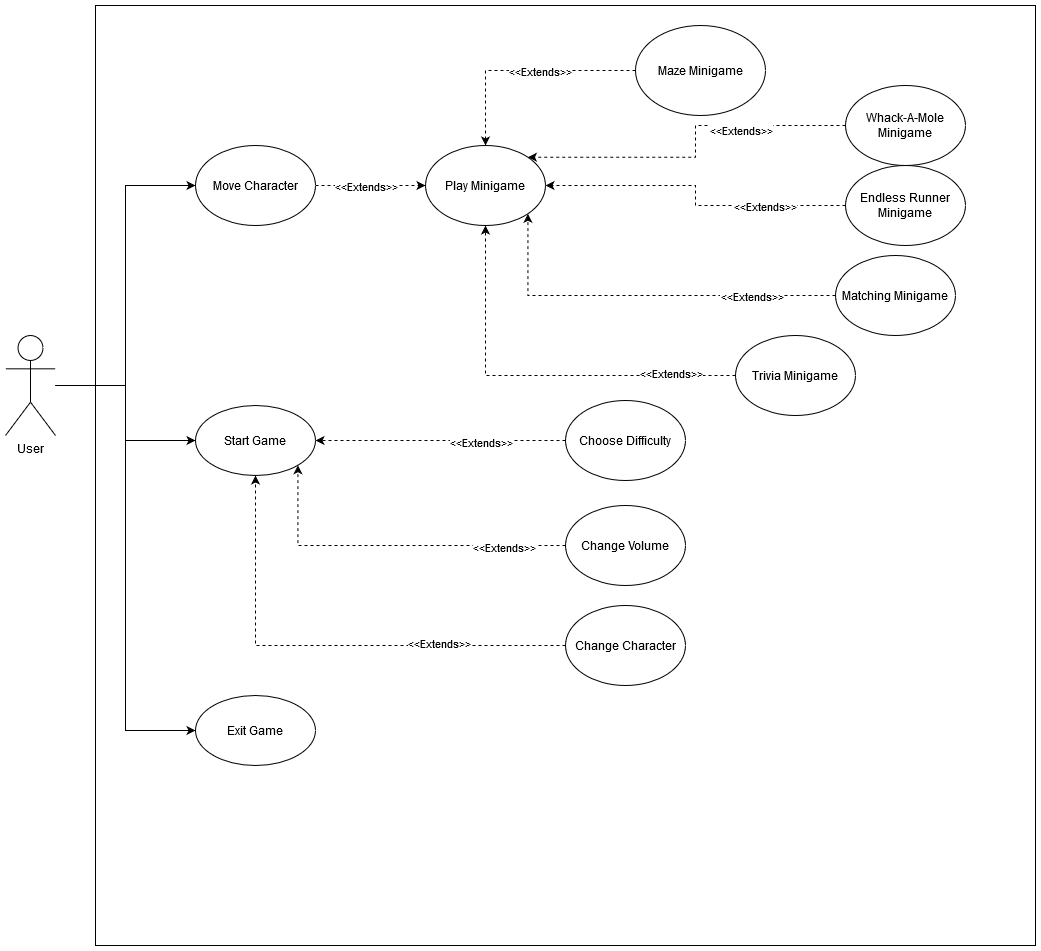
\includegraphics[width=1\textwidth]{figures/usecase.png}
    \caption{Use Case Diagram of the Project}
\end{figure}
% End Section 3

\section{Functional Requirements}
\label{sec:functional_requirements}
% Begin Section 4
\begin{enumerate}[{BE}1.]
	\item  The user wants to move the player character
	\begin{enumerate}[{VP1}.1]
		\item User
			\begin{enumerate}
				\item The character must move in the correct direction based on the user's inputs by keyboard or mouse.
				\item The character must be fixed in the centre of the whole screen when moving.
				\item The scene must moving as the character moves.
				\item The system must show notification that a task is available when the character is close to a task point.
			\end{enumerate}
	\end{enumerate}
	\item The user wants to initiate a mini-game
	\begin{enumerate}[{VP2}.1]
		\item User
			\begin{enumerate}
			    \item The system must notify the user that a "part" of the ship has broken and the mini-game to fix that part is now available.
				\item The system must allow the user to move to the designated location of the mini-game.
				\item The system must use the user's movements to determine if they are in the range to activate the mini-game.
				\item The system must allow the user a means to interact with the location of the game.
			\end{enumerate}
	\end{enumerate}
	\item The user wants to win a mini-game.
	\begin{enumerate}[{VP3}.1]
		\item User
			\begin{enumerate}
				\item The system must allow the user to input a set of properties.
				\item The system must allow the user to submit a set of properties.
				\item The system must notify the user of their current in-game properties.
				\item The system must evaluate the user's actions to determine if they have won.
				\item The system must notify the user that they have won the game.
				\item The system must redirect the user to the core game screen.
				\item The system must add the mini-game to a list of all currently won mini-games.
			\end{enumerate}
	\end{enumerate}
	\item The user loses a mini-game.
	\begin{enumerate}[{VP4}.1]
		\item User
			\begin{enumerate}
				\item The system must allow the user to input a set of properties.
				\item The system must allow the user to submit a set of properties.
				\item The system must notify the user of their current in-game properties.
				\item The system must use the user's actions to determine if they have lost.
				\item The system must notify the user that they have lost the game.
				\item The system must change the values of the ship health value.
				\item If the the health value of the ship is 0 then the system must load the end game screen.
				\item If the the health value of the ship is greater than 0 the system must load the core game screen.
			\end{enumerate}
	\end{enumerate}
	\item The user closes the browser.
	\begin{enumerate}[{VP5}.1]
		\item User
			\begin{enumerate}
				\item The system must display an alarm window that requires the player to confirm the exit.
				\item The system shall not save players' records.
				\item The system must terminate if players choose to close the browser in the alarm window.
				\item The system must return to the previous scene if players do not choose to close the browser in the alarm window.
			\end{enumerate}
	\end{enumerate}
	
\end{enumerate}

% End Section 4

\section{Non-Functional Requirements}
\label{sec:non-functional_requirements}
% Begin Section 5
\subsection{Look and Feel Requirements}
\label{sub:look_and_feel_requirements}

\subsubsection{Appearance Requirements}
\label{ssub:appearance_requirements}
\begin{enumerate}[{LF}1. ]
	\item The game's appearance will be bold, clean, and futuristic.
	\item The game will have a consistent space-themed brand which will involve bold sans-serif fonts, high-contrast blacks, blues, and whites, along with sharp, squared-off buttons and menus.
	\item The game's design will help remind the user that they are interacting with a spaceship in the future.
\end{enumerate}

\subsubsection{Style Requirements}
\label{ssub:style_requirements}
\begin{enumerate}[{LF}1. ]
	\item The game will have a dark and mysterious feel since users are battling against a mysterious person who is sabotaging the ship.
	\item The game will make the user feel immersed in the game and feel like the fate of the spaceship is truly in their hands.
	\item The game will include appropriate spooky background music and space-age sound effects.
\end{enumerate}

\subsection{Usability and Humanity Requirements}
\label{sub:usability_and_humanity_requirements}
% Begin SubSection

\subsubsection{Ease of Use Requirements}
\label{ssub:ease_of_use_requirements}
% Begin SubSubSection
\begin{enumerate}[{UH}1. ]
    \item The game does not require any intricate keyboard presses or fast and precise mouse movements. 
    \item If there is a bug or error the users can submit problems directly to the development team through email.
\end{enumerate}
% End SubSubSection

\subsubsection{Personalization and Internationalization Requirements}
\label{ssub:personalization_and_internationalization_requirements}
% Begin SubSubSection
\begin{enumerate}[{UH}1. ]
	\item The game will only have one language option of English. 
	\item The user can customize the sound of the game through the web-app 
	\item The user can change the name and the look of the character they use to play the game. 
\end{enumerate}
% End SubSubSection

\subsubsection{Learning Requirements}
\label{ssub:learning_requirements}
% Begin SubSubSection
\begin{enumerate}[{UH}1. ]
	\item User will be immediately able to use the software.
	\item Mechanisms will be in place to instruct the user of what to do in specific areas of the game.
\end{enumerate}
% End SubSubSection

\subsubsection{Understandability and Politeness Requirements}
\label{ssub:understandability_and_politeness_requirements}
% Begin SubSubSection
\begin{enumerate}[{UH}1. ]
	\item The tools used to instruct the user will be intuitive and easy to understand
	\item There will be a brief description of how to complete a mini-game before the user starts it.
	\item Any symbol used to help instruct the user will be associated to its cultural meaning
\end{enumerate}
% End SubSubSection

\subsubsection{Accessibility Requirements}
\label{ssub:accessibility_requirements}
% Begin SubSubSection
\begin{enumerate}[{UH}1. ]
	\item System will follow guidelines for correct colour contrast ratio for text to the background as stated in the WCAG ~\cite{wcag}
	%is there any accessibility functions that comes from our game not provided by the browser itself ?
\end{enumerate}
% End SubSubSection

% End SubSection

\subsection{Performance Requirements}
\label{sub:performance_requirements}
% Begin SubSection

\subsubsection{Speed and Latency Requirements}
\label{ssub:speed_and_latency_requirements}
% Begin SubSubSection
\begin{enumerate}[{PR}1. ]
	\item The average response time between player input and game response should be less than 0.25 seconds. 
	\item Users deem a product as unresponsive to use if the program reacts slowly on a consistent basis.
    \item The maximum response time between player input and game response should be no more than 1.5 seconds.
\end{enumerate}
% End SubSubSection

\subsubsection{Safety-Critical Requirements}
\label{ssub:safety_critical_requirements}
% Begin SubSubSection
\begin{enumerate}[{PR}1. ]
	\item The server hosting must be stable in order to ensure that the game does not restart, causing the player to restart the game as they lose all current progress. 
	\item The game is not being designed on an account-based system to save checkpoints, and users must complete the game in a single server session.
\end{enumerate}
% End SubSubSection

\subsubsection{Precision or Accuracy Requirements}
\label{ssub:precision_or_accuracy_requirements}
% Begin SubSubSection
\begin{enumerate}[{PR}1. ]
	\item The performance time must be within 30 percent of the expected time in order to deem the system to be accurate. 
	\item Repeated trials of 5 must show task performance times to be within 20 percent of each other in order to deem the system to be precise.
\end{enumerate}
% End SubSubSection

\subsubsection{Reliability and Availability Requirements}
\label{ssub:reliability_and_availability_requirements}
% Begin SubSubSection
\begin{enumerate}[{PR}1. ]
	\item The availability of the application is dependent on the status of the hosting service we are to use. 
	\item Reliability will be ensured by requiring at least 20 unit test cases for each component (mini-game) to confirm the software will operate as required.
\end{enumerate}
% End SubSubSection

\subsubsection{Robustness or Fault-Tolerance Requirements}
\label{ssub:robustness_or_fault_tolerance_requirements}
% Begin SubSubSection
\begin{enumerate}[{PR}1. ]
	\item The project must require error-based test cases for each component (mini-game) in order to lower the percentage of failures on invalid inputs. 
	\item Robustness related to the server stability must also be tested by checking performance under maximum user load.
\end{enumerate}
% End SubSubSection

\subsubsection{Capacity Requirements}
\label{ssub:capacity_requirements}
% Begin SubSubSection
\begin{enumerate}[{PR}1. ]
	\item The system shall be able to support 40 simultaneous users. This is highly dependent on the hosting service that will be used.
\end{enumerate}
% End SubSubSection

\subsubsection{Scalability or Extensibility Requirements}
\label{ssub:scalability_or_extensibility_requirements}
% Begin SubSubSection
\begin{enumerate}[{PR}1. ]
	\item The project mini-games will be created to be independent components to the core functionality, allowing future additions and scalability where developers can include more mini-games.
\end{enumerate}
% End SubSubSection

\subsubsection{Longevity Requirements}
\label{ssub:longevity_requirements}
% Begin SubSubSection
\begin{enumerate}[{PR}1. ]
	\item It can be expected for the web application to make use of \textbf{APIs} in order to implement one or more of the mini-games. 
	\item External \textbf{APIs} would be expected to continue functioning for the game to remain functional. 
	\item If external \textbf{APIs} are shut down unexpectedly, the game will no longer work.
\end{enumerate}
% End SubSubSection

% End SubSection

\subsection{Operational and Environmental Requirements}
\label{sub:operational_and_environmental_requirements}
% Begin SubSection

\subsubsection{Expected Physical Environment}
\label{ssub:expected_physical_environment}
% Begin SubSubSection
\begin{enumerate}[{OE}1. ]
	\item The game will be able to run on browsers in both desktops and laptops with installation of Windows 10, MacOS or Linux environment.
\end{enumerate}
% End SubSubSection

\subsubsection{Requirements for Interfacing with Adjacent Systems}
\label{ssub:requirements_for_interfacing_with_adjacent_systems}
% Begin SubSubSection
\begin{enumerate}[{OE}1. ]
	\item The game will be able to run on different browsers.
\end{enumerate}
% End SubSubSection

\subsubsection{Productization Requirements}
\label{ssub:productization_requirements}
% Begin SubSubSection
\begin{enumerate}[{OE}1. ]
	\item There is no specific productization requirements of this game.
\end{enumerate}
% End SubSubSection

\subsubsection{Release Requirements}
\label{ssub:release_requirements}
% Begin SubSubSection
\begin{enumerate}[{OE}1. ]
	\item There is no specific release requirements of this game.
\end{enumerate}
% End SubSubSection

% End SubSection

\subsection{Maintainability and Support Requirements}
\label{sub:maintainability_and_support_requirements}


\subsubsection{Maintenance Requirements}
\label{ssub:maintenance_requirements}
\begin{enumerate}[{MS}1. ]
% time to make changes, who makes changes, ease of changes
	\item All team members will be required to make changes over the lifespan of the game.
	\item Errors or issues that are found in the code that will need to be remedied.
	\item Critical priority bugs will need to be fixed before low priority bugs.
	\item New levels, new mini-games, new characters, or any other new additions must be added to the game over time.
	\item New features must be finished in order to meet release timelines.
\end{enumerate}

\subsubsection{Supportability Requirements}
\label{ssub:supportability_requirements}
\begin{enumerate}[{MS}1. ]
	\item The game will show a tutorial on first load showing the user what the controls are, what the objective is, and how to play. 
	\item A contact email will be displayed on the game's main page to accept user feedback and to provide support.
\end{enumerate}

\subsubsection{Adaptability Requirements}
\label{ssub:adaptability_requirements}
\begin{enumerate}[{MS}1. ]
	\item The game will be released as a web app.
	\item The game will be playable in the browser on a wide variety of platforms.
\end{enumerate}

\subsection{Security Requirements}
\label{sub:security_requirements}
% Begin SubSection

\subsubsection{Access Requirements}
\label{ssub:access_requirements}
% Begin SubSubSection
\begin{enumerate}[{SR}1. ]
	\item The game shall be accessible to all users that can access a web browser
	\item The game shall be accessible to all users whereby a geographical location's jurisdiction permits access
	\item Users shall be able to access "unlockable" cosmetic items upon successful completion of the game.
\end{enumerate}
% End SubSubSection

\subsubsection{Integrity Requirements}
\label{ssub:integrity_requirements}
% Begin SubSubSection
\begin{enumerate}[{SR}1. ]
	\item All data pertaining to the game shall only be accessible to the developers of the game.
\end{enumerate}
% End SubSubSection

\subsubsection{Privacy Requirements}
\label{ssub:privacy_requirements}
% Begin SubSubSection
\begin{enumerate}[{SR}1. ]
	\item Not applicable for this application.
\end{enumerate}
% End SubSubSection

\subsubsection{Audit Requirements}
\label{ssub:audit_requirements}
% Begin SubSubSection
\begin{enumerate}[{SR}1. ]
	\item The performance of the game shall be checked to ensure the game meets the specified performance requirements
	\item Any and all bug fixes and new features shall be tested to ensure the game continues to conform to all requirements specified in the \textbf{SRS}.
	\item The usability of the game shall be checked to ensure the game is still accessible and understandable for its users
\end{enumerate}
% End SubSubSection

\subsubsection{Immunity Requirements}
\label{ssub:immunity_requirements}
% Begin SubSubSection
\begin{enumerate}[{SR}1. ]
	\item Not applicable for this application.
\end{enumerate}
% End SubSubSection

% End SubSection

\subsection{Cultural and Political Requirements}
\label{sub:cultural_and_political_requirements}
% Begin SubSection

\subsubsection{Cultural Requirements}
\label{ssub:cultural_requirements}
% Begin SubSubSection
\begin{enumerate}[{CP}1. ]
	\item The game will not use any content that may be offensive to any culture. 
\end{enumerate}
% End SubSubSection

\subsubsection{Political Requirements}
\label{ssub:political_requirements}
% Begin SubSubSection
\begin{enumerate}[{CP}1. ]
	\item The game will not incorporate any character of a political nature.
	\item The game will not use any language that is politically driven.
\end{enumerate}
% End SubSubSection

% End SubSection

\subsection{Legal Requirements}
\label{sub:legal_requirements}
% Begin SubSection

\subsubsection{Compliance Requirements}
\label{ssub:compliance_requirements}
% Begin SubSubSection
\begin{enumerate}[{LR}1. ]
    \item The game will adhere to all data privacy laws and regulations of the countries by which the game is operated in. (i.e., PIPEDA-Canada, GDPR-EU) ~\cite{PIPEDA-CA} ~\cite{GDPR-EU}
	\item The game will inform its users of any personal identifying data that may be collected, and its purposes.
\end{enumerate}
% End SubSubSection

\subsubsection{Standards Requirements}
\label{ssub:standards_requirements}
% Begin SubSubSection
\begin{enumerate}[{LR}1. ]
	\item The game will comply with all age-restriction standards of the geographical locations by which the game is operable in (i.e., ESRB ratings). 
\end{enumerate}
% End SubSubSection

% End SubSection

% End Section 5
\newpage
\appendix
\section{Division of Labour}
\label{sec:division_of_labour}
% Begin Section

\begin{table}[h]
    \centering
    \begin{tabular}{|c|c|c|}
    \hline
        \textbf{Name} & \textbf{Contributed Part} & \textbf{Signature} \\
        \hline
        Benson & Section 2.2, 2.3, 4, 5 & 
\includegraphics[width=0.3\textwidth]{signatures/bensonsignature.JPG}\\
        \hline
        Graeme & Section 1.3, 1.4, 2.6, 4, 5 & 
\includegraphics[width=0.3\textwidth]{signatures/graeme_signature.png} \\
        \hline
        Jiawei & Section 2.1, 4, 5 & 
\includegraphics[width=0.3\textwidth]{signatures/Signature_Jiawei.PNG}\\
        \hline
        Nick & Section 1.1, 2.2, 3, 4, 5 & 
\includegraphics[width=0.3\textwidth]{signatures/nick signature.PNG} \\
        \hline
        Rupinder & Section 1.2, 2.1, 2.4, 2.5, 4, 5 & 
\includegraphics[width=0.3\textwidth]{signatures/Rupinder Signature.png}\\
        \hline
    \end{tabular}
    \caption{Division of Labour}
    \label{tab:my_label}
\end{table}

% End Section
\end{document}
%------------------------------------------------------------------------------